\subsection{Variance-Based Definition of $p_j$}
\label{sec:variance-p}

$p_j$ is meant to reward recipients whose opening is \emph{informative}
about others, in the sense of informativeness used throughout active
learning. The original definition,
$p_j = \frac{1}{m-1}\sum_{i\ne j}\Sigma_{j,i}$, rewards recipients that
raise the \emph{average level} of other recipients' $f$-scores --- which is
not the same as reducing uncertainty about them. We instead reward maximal
\emph{spread} induced across other recipients' scores, following
variance-based exploration bonuses in the multi-armed bandit literature
\citep{audibert2009exploration}:
\begin{equation}
\label{eq:p-variance}
p_j = \frac{4}{m-1}\sum_{i\ne j}\big(\Sigma_{j,i} - \bar\Sigma_{j:}\big)^2,
\qquad
\bar\Sigma_{j:} = \frac{1}{m-1}\sum_{i\ne j}\Sigma_{j,i}.
\end{equation}
This is the variance of $\Sigma_{j,:}$ (excluding $j$), scaled by $4$ so
that the maximum possible variance of a Bernoulli variable (0.25) maps to
1, keeping $p_j \in [0,1]$.
The two definitions therefore favor different recipients, which is visible in
the rows of $\Sigma$ themselves (Figure~\ref{fig:sigma-rows}c). Writing
$p^{\mathrm{mean}}$ and $p^{\mathrm{var}}$ for the original and the
variance-based definition, the recipient maximizing $p^{\mathrm{mean}}$ has a
unimodal row with a peak at $1$ ($p^{\mathrm{mean}}=0.82$,
$p^{\mathrm{var}}=0.17$), whereas the recipient maximizing $p^{\mathrm{var}}$
has a bimodal row with peaks at $0$ and $1$ ($p^{\mathrm{var}}=0.70$,
$p^{\mathrm{mean}}=0.44$).

\begin{figure*}[t]
\centering
\newlength{\pww}\newlength{\phh}
\setlength{\pww}{0.32\textwidth}\addtolength{\pww}{-2\fboxsep}\addtolength{\pww}{-2\fboxrule}
\setlength{\phh}{1.114\pww}% matches the 158.4x176.4pt aspect of panel (c)
\begin{minipage}[b]{0.32\textwidth}
\centering
\fbox{\parbox[c][\phh][c]{\pww}{\centering\small\color{gray}Placeholder\\(figure a)}}\\[2pt]
{\small (a)}
\end{minipage}\hfill
\begin{minipage}[b]{0.32\textwidth}
\centering
\fbox{\parbox[c][\phh][c]{\pww}{\centering\small\color{gray}Placeholder\\(figure b)}}\\[2pt]
{\small (b)}
\end{minipage}\hfill
\begin{minipage}[b]{0.32\textwidth}
\centering
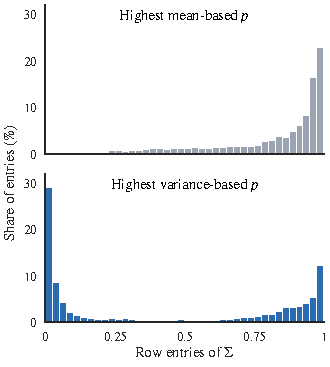
\includegraphics[width=\linewidth]{figures/fig_p_sigma_rows.pdf}\\[2pt]
{\small (c)}
\end{minipage}
\caption{[Placeholder: caption for panels (a) and (b).]
\textbf{(c)} Distribution of the entries of the row of $\Sigma$ belonging to the
recipient with the highest $p$ under the mean-based definition (top) and under
the variance-based definition (bottom).}
\label{fig:sigma-rows}
\end{figure*}
